\documentclass[conference]{IEEEtran}
\usepackage[utf8]{inputenc}
\usepackage{graphicx}
\usepackage{amsmath}
\usepackage{cite}
\usepackage{float}

\title{Migración en El Salvador: Una Perspectiva Socioeconómica}
\author{\IEEEauthorblockN{Natanael de Jesús Rivera Hernández}
\IEEEauthorblockA{Departamento de Ciencias Sociales\\
Universidad de El Salvador\\
Email: natanael.rivera@example.com}
\and
\IEEEauthorblockN{Rene Salvador Cardoza Godínez}
\IEEEauthorblockA{Departamento de Ciencias Sociales\\
Universidad de El Salvador\\
Email: rene.cardoza@example.com}
}

\begin{document}
\maketitle

\begin{abstract}
La migración en El Salvador ha tenido un impacto significativo en su desarrollo social, económico y político. Este artículo analiza las causas principales de la migración, sus efectos en la sociedad salvadoreña y las posibles soluciones para mitigar las consecuencias negativas. Se incluyen datos estadísticos, gráficos y fórmulas que refuerzan el análisis.
\end{abstract}

\section{Introducción}
La migración ha sido un fenómeno constante en El Salvador, influenciado por factores como la violencia, la falta de oportunidades económicas y los desastres naturales. Según estudios recientes \cite{unmigration2021}, un porcentaje significativo de la población salvadoreña reside en el extranjero, principalmente en los Estados Unidos.

\section{Causas de la Migración}
Entre las principales causas de la migración en El Salvador se encuentran:
\begin{itemize}
    \item La violencia de las pandillas.
    \item La pobreza y el desempleo.
    \item Los desastres naturales como huracanes y terremotos.
\end{itemize}

\section{Impacto Socioeconómico}
La migración tiene efectos positivos y negativos en la economía salvadoreña. A continuación, se presentan dos tablas que muestran datos sobre remesas y población migrante.

\subsection{Tabla de Remesas Recibidas}
\begin{table}[H]
\caption{Remesas recibidas en El Salvador (2020-2023).}
\label{table_remesas}
\centering
\begin{tabular}{|c|c|c|}
\hline
Año & Remesas (millones de \$) & Variación (\%) \\ \hline
2020 & 5700 & -5.0 \\ \hline
2021 & 6500 & 14.0 \\ \hline
2022 & 7000 & 7.7 \\ \hline
2023 & 7300 & 4.3 \\ \hline
\end{tabular}
\end{table}

\subsection{Distribución de Migrantes}
\begin{table}[H]
\caption{Distribución de migrantes salvadoreños por región.}
\label{table_migrantes}
\centering
\begin{tabular}{|l|c|}
\hline
Región & Porcentaje (\%) \\ \hline
América del Norte & 85 \\ \hline
América Latina & 10 \\ \hline
Europa & 4 \\ \hline
Asia y Oceanía & 1 \\ \hline
\end{tabular}
\end{table}

\section{Análisis Matemático}
Se pueden modelar las remesas recibidas utilizando una progresión geométrica:
\begin{equation}
R_n = R_0 \cdot (1 + g)^n, \quad \text{donde } g = \text{tasa de crecimiento}.
\label{eq:remesas}
\end{equation}

Además, la distribución de migrantes puede representarse por un sistema de ecuaciones para las distintas regiones:
\begin{equation}
P_{\text{total}} = P_{\text{América del Norte}} + P_{\text{América Latina}} + P_{\text{Europa}} + P_{\text{Asia y Oceanía}}.
\label{eq:distribucion}
\end{equation}

\section{Representación Visual}
\subsection{Imágenes de Apoyo}
En la Figura~\ref{fig:migrantes}, se presenta un gráfico que ilustra las rutas migratorias más comunes desde El Salvador.

\begin{figure}[H]
\centering
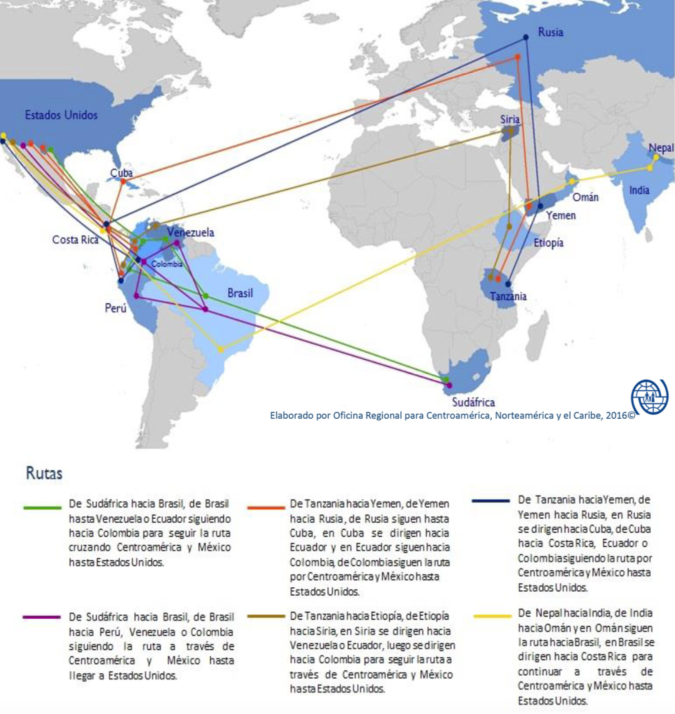
\includegraphics[width=0.45\textwidth]{imagenes/rutas_migratorias.png}
\caption{Rutas migratorias desde El Salvador.}
\label{fig:migrantes}
\end{figure}

\subsection{Imagen a Dos Columnas}
\begin{figure*}[t]
\centering

\includegraphics[width=\textwidth]{imagenes/impacto_remesas.png}
\caption{Impacto de las remesas en la economía salvadoreña.}
\label{fig:remesas}
\end{figure*}

\section{Conclusión}
La migración en El Salvador es un fenómeno complejo con raíces profundas en problemas estructurales. Sin embargo, con estrategias adecuadas, se pueden maximizar los beneficios y minimizar los efectos negativos.

\section*{Agradecimientos}
Agradecemos a la Universidad de El Salvador por su apoyo en la realización de este estudio.

\bibliographystyle{IEEEtran}
\bibliography{referencias}

\end{document}
